\documentclass[fleqn, 10pt]{article}

% Paquetes necesarios
\usepackage[utf8]{inputenc}
\usepackage[spanish]{babel}
\usepackage{amsthm}
\usepackage{nccmath} %Para centrar ecuaciones
\usepackage{enumitem}
\usepackage{graphicx}
\usepackage{verbatim}




\DeclareMathAlphabet{\pazocal}{OMS}{zplm}{m}{n}
\newcommand{\Lb}{\pazocal{L}}


\theoremstyle{plain}
\newtheorem{proposicion}{Proposición}

\theoremstyle{definition}
\newtheorem{definition}{Definición}[section]
\newtheorem{example}{Ejemplo}[section]

%Definimos el título
\title{Teoría de Autómatas y Lenguajes Formales\\[.4\baselineskip]Práctica 2: Autómatas en JFLAP}
\author{Alba Robles Morales}
\date{27/10/2022}



%Comienzo del documento
\begin{document}

%Generamos el título
\maketitle

\section{Considera un lenguaje sobre un alfabeto\{a,b\} que solo contenga la cadena  'a'. }

\subsection{Construye un autómata finito determinista que reconozca este lenguaje y rechaze todas las cadenas que no pertenecen a él.}
\subsection{ Testea el autómata que has creado introduciendo 6 cadenas}

\begin{equation}
 M= (\{q0,q1,q2\},\{a,b\},\{(q0,a,q1),(q0,b,q2),(q1,a,q2)(q1,b,q2),(q2,a,q2),(q2,b,q2)\},q0, \{q1\}) 
\end{equation}

\begin{equation}
(q0,a)\vdash(q1, \epsilon)\wedge q1 \in F \Rightarrow a \in \pazocal{L}(M)
\end{equation}
\begin{equation}
(q0,aa)\vdash(q1, a)\vdash(q2, \epsilon)\wedge q2 \notin F \Rightarrow aa \notin \pazocal{L}(M)
\end{equation}

 
\begin{center}
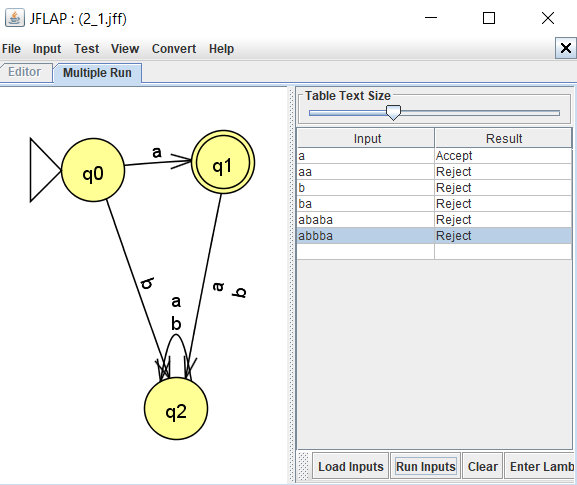
\includegraphics[width=9cm, height=6cm]{2_1.png}
\end{center}

\section{También hacerlo en Octave, describiendo el JSON dentro de un entorno "verbatim" de \LaTeX.}
\begin{verbatim}
 {
	"name" : "a",
	"representation":{
	"K": ["qo","q1","q2"],
	"A": ["a","b"],
	"s": "q0",
	"F": ["q1"],
	"t":[["q0","a","q1"],
	     ["q0","b","q2"],
	     ["q1","a","q2"]
	     ["q1","b","q2"],
	     ["q2","a","q2"],
	     ["q2","b","q2"]]
	}
}
\end{verbatim}





\end{document}